\documentclass{article}
\usepackage{tikz, comment}
\usepackage{pifont}
\usepackage{fontspec, pgfplots}
\usetikzlibrary{arrows, decorations.markings, decorations.pathreplacing}
\begin{comment}
:Title: Not defined yet
:Tags: cross product;end behavior;triple (scalar) product;pappus&#146;s theorem, theorem of pappus;perimeter
:Prob: 0.4848;0.4364;0.4262;0.4147;0.3936
:Author: Prof.Hu Ji-shan, HKUST
:Slug: No name yet

Description Here.........
\end{comment}
\begin{document}\centering 

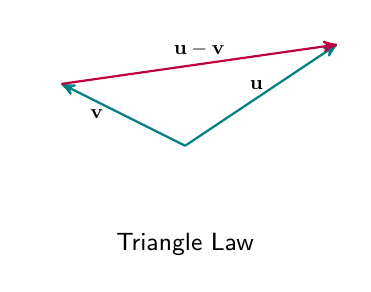
\begin{tikzpicture}[>=latex,xscale=.5*1, yscale=.5*1][font=\sf\small] 

\clip[] (-4, -3) rectangle (4, 3);

\draw[teal, thick, ->, >=stealth'] (0, 0) -- ({3*9/7}, {2*9/7}) node[black, left, pos=0.6, xshift=-2, yshift=0, scale=0.8]{${\bf u}$};

\draw[teal, thick, ->, >=stealth'] (0, 0) -- ({-2*11/7}, {1*11/7}) node[black, left, pos=0.6, xshift=0, yshift=-2, scale=0.8]{${\bf v}$};

\draw[purple, thick, ->, >=stealth'] ({-2*11/7}, {1*11/7}) -- ({3*9/7}, {2*9/7}) node[black, above, midway, pos=0.5, xshift=0, yshift=0, scale=0.8]{${\bf u-v}$};

\node at (0, -2.5) {$\hbox{Triangle Law}$};

\end{tikzpicture}\hskip1cm
\end{document}